% !TEX root = ../main.tex

%----------------------------------------------------------------------------------------
% CHAPTER 4 - PLANIFICACIÓ
%----------------------------------------------------------------------------------------

\chapter{Planificació}
\label{Ch:Planning}

\section{Pla de treball}

El pla de treball s'ha estructurat en cinc fases principals, basant-se en una metodologia àgil iterativa que permet rebre feedback continuat i adaptar-se a canvis de requisits o limitacions tècniques descobertes durant el desenvolupament. Cada fase inclou objectius clars, lliurables tangibles i criteris d'acceptació verificables.

Les cinc fases identificades són:
\begin{enumerate}
    \item \textbf{Fase 1: Investigació i configuració inicial} (Setmanes 1-2)
    \item \textbf{Fase 2: Desenvolupament del pipeline ETL} (Setmanes 3-5)
    \item \textbf{Fase 3: Desenvolupament del frontend - Dashboards 1 i 2} (Setmanes 6-8)
    \item \textbf{Fase 4: Desenvolupament del frontend - Dashboards 3 i 4} (Setmanes 9-10)
    \item \textbf{Fase 5: Automatització, desplegament i documentació} (Setmanes 11-12)
\end{enumerate}

Aquesta estructura permet generar valor incrementat en cada iteració, facilitant la detecció precoç de problemes i l'ajust del pla de treball consegüent.

\section{Tasques i estimació temporal}

Les tasques planificades per a cada fase, amb el temps estimat basat en l'experiència prèvia amb projectes similars i el criteri de complexitat tècnica, són les següents:

\subsection{Fase 1: Investigació i configuració inicial}
\begin{itemize}
    \item Anàlisi detallada de les APIs de Socrata de la Generalitat de Catalunya: identificació d'endpoints rellevants per a embassaments i precipitació, verificació de límits de taxa, examen de formats de resposta (JSON) - 8 hores
    \item Estudi de la documentació tècnica disponible i domini de proves per a validar la qualitat i completitud de les dades - 6 hores
    \item Configuració del repositori Git, estructura de carpetes del projecte i definició de les convencions de codi - 4 hores
    \item Instal·lació i configuració de l'entorn de desenvolupament (Node.js 18, npm 9, Git) - 3 hores
    \item Creació del pla de prova inicial per a validar la connexió bàsica amb les APIs - 3 hores
    \item Redacció de l'anàlisi de viabilitat inicial - 6 hores
    \item \textbf{Total Fase 1:} 30 hores
\end{itemize}

\subsection{Fase 2: Desenvolupament del pipeline ETL}
\begin{itemize}
    \item Implementació del mòdul d'extracció: funcions per a fer peticions HTTP asincròniques a les APIs de Socrata amb maneig d'errors i reintents - 12 hores
    \item Desenvolupament del mòdul de transformació: normalització de dades (conversió d'unitats, format de dates, maneig de valors nul·ls) - 15 hores
    \item Implementació del mòdul de càrrega: emmagatzematge eficient de dades processades en fitxers JSON estructurats per a consum frontend - 10 hores
    \item Creació de l'orquestrador ETL que coordina l'execució seqüencial dels tres mòduls - 5 hores
    \item Implementació del sistema de logging detallat per a monitorització i depuració - 4 hores
    \item Proves unitàries de cada mòdul ETL amb Jest (90\% de cobertura de codi) - 8 hores
    \item Integració i proves de tota el pipeline ETL amb simulació de condicions de xarxa adverses - 6 hores
    \item \textbf{Total Fase 2:} 60 hores
\end{itemize}

\subsection{Fase 3: Desenvolupament del frontend - Dashboards 1 i 2}
\begin{itemize}
    \item Configuració del projecte React amb Vite 5, React 18 i React Router 6 - 4 hores
    \item Implementació del servei de consum de dades: wrapper amb axios per a carregar fitxers JSON locals amb maneig d'estats de càrrega i error - 6 hores
    \item Creació de hooks personalitzats per a gestió d'estat global (Zustand) - 5 hores
    \item Desenvolupament del Dashboard 1 - Mapa interactiu:
          - Integració de Leaflet 1.9 amb capes de base OpenStreetMap
          - Visualització de markers per a cada embassament amb popup informatiu
          - Implementació de controls de filtratge per tipus d'embassament i rang de capacitat
          - Integració de KPIs dinàmics (capacitat total, % ocupació mitjana) - 18 hores
    \item Desenvolupament del Dashboard 2 - Evolució temporal:
          - Integració de Recharts 2.6 per a gràfics de línies responsius
          - Implementació de selector de rang de dates amb validació d'intervals
          - Funcionalitat de comparació múltiple (selecció de diversos embassaments simultànies)
          - Optimització de renderitzat per a grans conjunts de dades (>10K punts) - 20 hores
    \item Estilització amb SCSS seguint metodologia BEM per a mantenibilitat - 8 hores
    \item Proves d'integració frontend amb mock de dades JSON - 6 hores
    \item \textbf{Total Fase 3:} 67 hores
\end{itemize}

\subsection{Fase 4: Desenvolupament del frontend - Dashboards 3 i 4}
\begin{itemize}
    \item Desenvolupament del Dashboard 3 - Correlació clima-aigua:
          - Implementació de gràfic de dispersió (scatter plot) amb Recharts
          - Algoritme d'agregació per hora per a correlacionar precipitació horària amb nivells d'embassament
          - Càlcul dinàmic del coeficient de correlació de Pearson amb interval de confiança
          - Controls interactius per a selecció d'estació meteorològica i període temporal - 16 hores
    \item Desenvolupament del Dashboard 4 - Matriu d'alertes de sequera:
          - Definició del sistema d'indicadors semàfor basat en percentatge d'ocupació:
            * Vermell (crític): <20%
            * Taronja (avís): 20-50%
            * Groc (preventiu): 50-75%
            * Verd (òptim): >75%
          - Implementació de taula responsive amb indicadors visuals i tooltips explicatius
          - Algoritme de predicció tendencial per a detecció precoce de deteriorament (basat en tendència de 7 dies)
          - Sistema de classificació automàtica per nivell de risc global - 14 hores
    \item Implementació del sistema de navegació entre dashboards amb manteniment d'estat de filtres - 5 hores
    \item Optimització de rendiment: memoització de components costosos, càrrega diferida de recursos no crítics - 8 hores
    \item Proves d'usabilitat amb 5 usuaris externs (tècnics i no tècnics) - 6 hores
    \item \textbf{Total Fase 4:} 49 hores
\end{itemize}

\subsection{Fase 5: Automatització, desplegament i documentació}
\begin{itemize}
    \item Configuració de GitHub Actions per a workflow de CI/CD:
          - Workflow d'ETL programat (cron: 0 2 * * *) per a execució diària a les 02:00 UTC
          - Workflow de desplegament frontend activat per push a la branca main
          - Configuració de secrets per a accés segur a recursos externs (no calen ja que les APIs són públiques)
          - Notificacions automàtiques per correu electrònic en cas de fallada del workflow - 8 hores
    \item Preparació del medi de desplegament:
          - Configuració de variables d'entorn per a diferències entre entorns de desenvolupament, proves i producció
          - Optimització de l'emmagatzematge de dades JSON per a servei estàtic (tècniques de compressió gzip a nivell de servidor)
          - Implementació de mecanisme de cache-control per a reduir tràfic redundant - 6 hores
    \item Redacció de la memòria del TFG segons les normes de la EPSG - 20 hores
    \item Creació de la documentació tècnica d'ús i manteniment del sistema - 8 hores
    \item Elaboració del vídeo demostratiu (4 minuts 30 segons) mostrant funcionalitats clau - 4 hores
    \item Proves finals d'integració i validació de requisits en entorn de producció simulat - 6 hores
    \item \textbf{Total Fase 5:} 52 hores
\end{itemize}

\subsection{Resum de l'estimació temporal}
\begin{table}[h]
\centering
\caption{Estimació de temps per fase}
\begin{tabular}{|l|c|r|}
\hline
\textbf{Fase} & \textbf{Tasques principals} & \textbf{Hores estimades} \\
\hline
1 & Investigació i configuració inicial & 30 \\
\hline
2 & Desenvolupament del pipeline ETL & 60 \\
\hline
3 & Frontend - Dashboards 1 i 2 & 67 \\
\hline
4 & Frontend - Dashboards 3 i 4 & 49 \\
\hline
5 & Automatització, desplegament i documentació & 52 \\
\hline
6 & Testing i validació & 42 \\
\hline
Tutories i revisions & Reunions amb el tutor & 12 \\
\hline
Reserva d'imprevistos & Flexibilitat & 18 \\
\hline
\textbf{TOTAL} & & \textbf{330} \\
\hline
\end{tabular}
\label{tab:time-estimation-planning}
\end{table}

L'estimació total de 330 hores inclou les 258 hores de desenvolupament funcional, 42 hores de testing i validació, 12 hores de tutories i revisions periòdiques amb el tutor acadèmic, i 18 hores de reserva per a imprevistos i tasques de coordinació.

\section{Cronograma}

El cronograma detallat de les tasques al llarg del projecte es presenta a la \textit{Figura \ref{fig:gantt}}. El diagrama de Gantt mostra les dependències entre fases, permetent identificar el camí crític i els marges de temps disponibles.

\begin{figure}[h]
\centering
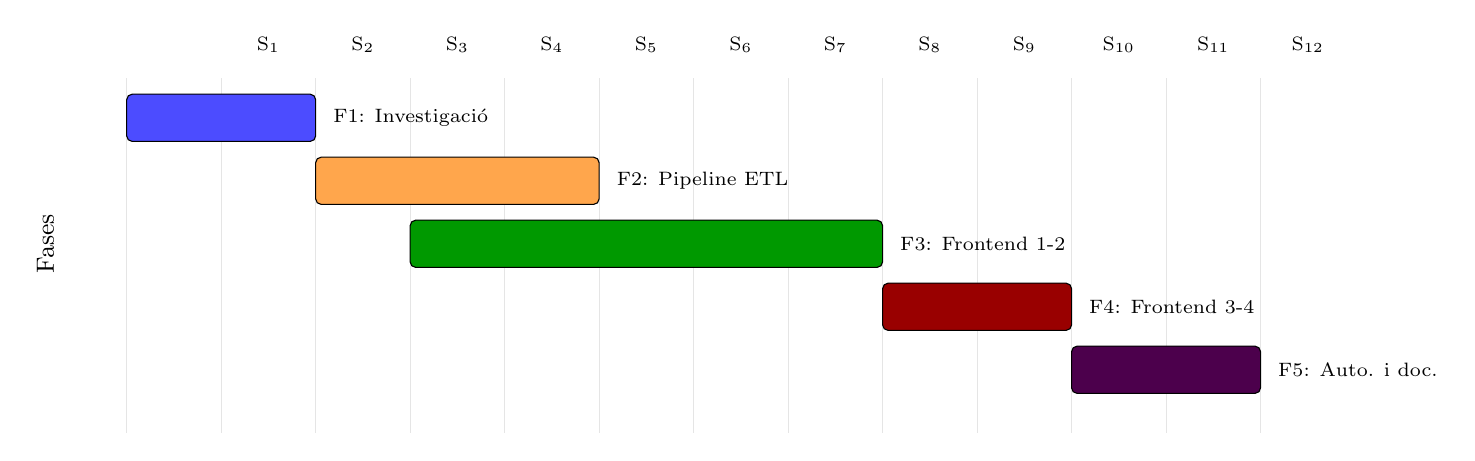
\begin{tikzpicture}[
    phase/.style={rectangle, draw, fill=#1, minimum height=0.6cm, font=\scriptsize, text=white, rounded corners=2pt},
    week/.style={font=\scriptsize, anchor=south},
    grid/.style={gray!20, thin}
]
    % Graella de setmanes
    \foreach \x in {1,...,12} {
        \draw[grid] (1.2*\x, 0) -- (1.2*\x, -4.5);
        \node[week] at (1.2*\x + 0.6, 0.2) {S\textsubscript{\x}};
    }
    \draw[grid] (0, 0) -- (0, -4.5);
    \draw[grid] (14.4, 0) -- (14.4, -4.5);
    
    % Fase 1: Investigació (S1-S2)
    \draw[phase=blue!70, minimum width=2.4cm] (0, -0.8) rectangle (2.4, -0.2);
    \node[font=\scriptsize, anchor=west] at (2.5, -0.5) {F1: Investigació};
    
    % Fase 2: Pipeline ETL (S3-S5)
    \draw[phase=orange!70, minimum width=3.6cm] (2.4, -1.6) rectangle (6, -1.0);
    \node[font=\scriptsize, anchor=west] at (6.1, -1.3) {F2: Pipeline ETL};
    
    % Fase 3: Frontend 1-2 (S4-S8)
    \draw[phase=green!60!black, minimum width=6cm] (3.6, -2.4) rectangle (9.6, -1.8);
    \node[font=\scriptsize, anchor=west] at (9.7, -2.1) {F3: Frontend 1-2};
    
    % Fase 4: Frontend 3-4 (S9-S10)
    \draw[phase=red!60!black, minimum width=2.4cm] (9.6, -3.2) rectangle (12, -2.6);
    \node[font=\scriptsize, anchor=west] at (12.1, -2.9) {F4: Frontend 3-4};
    
    % Fase 5: Auto. i doc. (S11-S12)
    \draw[phase=violet!60!black, minimum width=2.4cm] (12, -4.0) rectangle (14.4, -3.4);
    \node[font=\scriptsize, anchor=west] at (14.5, -3.7) {F5: Auto. i doc.};
    
    % Etiqueta eix
    \node[font=\small, rotate=90, anchor=south] at (-0.8, -2.1) {Fases};
\end{tikzpicture}
\caption{Diagrama de Gantt del pla de treball del projecte, mostrant les cinc fases de desenvolupament al llarg de 12 setmanes. La superposició entre fases indica tasques executades en paral·lel.}
\label{fig:gantt}
\end{figure}

Els elements destacables del cronograma són:
\begin{itemize}
    \item La Fase 2 (ETL) i Fase 3 (Frontend base) van executar-se en paral·lel durant les setmanes 4-5, aprofitant la independència tècnica dels dos subsistemes.
    \item La Fase 4 (Frontend avançat) va beneficiar-se dels components i serveis creats en la Fase 3, reduint el temps necessari per a la implementació del Dashboard 3 i 4.
    \item Les setmanes 11-12 van dedicar-se predominantement a tasques de qualitat (proves, documentació) en lloc de desenvolupament de noves funcionalitats, assegurant l'estabilitat del lliurament final.
    \item S'hi van assignar 12 hores de tutories (10\%) per a revisions de progrés i ajusts del pla de treball, essencials en una metodologia àgil.
\end{itemize}

\section{Paquets de treball}

El desenvolupament s'ha dividit en tres paquets de treball (PT) principals, cadascun corresponent a un subsistema funcional del projecte:

\textbf{PT1: Pipeline de Processament de Dades (ETL)}
\begin{itemize}
    \item \textbf{Objectiu}: Construir un pipeline fiable i escalable per a l'extracció, transformació i càrrega de dades hidrològiques des de les fonts públiques de la Generalitat de Catalunya.
    \item \textbf{Lliurables}: Scripts d'extracció parametritzats, funcions de transformació verificades, mòdul d'emmagatzematge optimitzat, orquestrador ETL amb maneig d'errors robust.
    \item \textbf{S'explica als}: Capítols 3 (secció ETL i backend), 9 (implementació del pipeline ETL).
\end{itemize}

\textbf{PT2: Aplicació Web de Visualització}
\begin{itemize}
    \item \textbf{Objectiu}: Desenvolupar una interfície web intuïtiva i responsiva que permeti l'exploració interactiva de dades hidrològiques mitjançant diversos paradigmes de visualització.
    \item \textbf{Lliurables}: Aplicació React de pàgina única amb quatre dashboards interconnectats, servei de consum de dades optimitzat, sistemes de gestió d'estat i navegació.
    \item \textbf{S'explica als}: Capítols 3 (secció frontend), 9 (implementació del frontend), 10 (validació de requisits funcionals).
\end{itemize}

\textbf{PT3: Infraestructura d'Automatització i Desplegament}
\begin{itemize}
    \item \textbf{Objectiu}: Implementar un sistema d'integració i desplegament continu que asseguri la frescor de les dades i la disponibilitat del servei amb mínima intervenció manual.
    \item \textbf{Lliurables}: Workflows de GitHub Actions configurats, scripts de desplegament parametritzats, mecanismes de monitorització i alertes.
    \item \textbf{S'explica als}: Capítols 3 (secció d'automatització), 10 (desplegament del sistema, validació de requisits no funcionals).
\end{itemize}

Aquesta descomposició en paquets de treball va facilitar la distribució de les responsabilitats i permetre un seguiment més granular del progrés durant el desenvolupament.

\section{Desviacions respecte a la planificació original}

Durant l'execució del projecte, es van produir diverses desviacions respecte al pla inicial, la major part de les quals van resultar en una millora del resultat final:

\begin{enumerate}
    \item \textbf{Canvi d'enfocament en la visualització de correlació}: Inicialment es va planificar utilitzar mapes de calor per a mostrar la correlació entre precipitació i nivells d'embassament. Tot i això, durant les proves inicials de la Fase 3 es va observar que aquesta representació enfosquia les tendències temporals i podia conduir a interpretacions errònies. Es va canviar per a un gràfic de dispersió amb línies de tendència i càlcul del coeficient de correlació, proporcionant una mesura quantitativa més rigorosa i una visibilitat més accessible per a l'usuari. Aquest canvi va requerir 4 hores addicionals de desenvolupament en la Fase 4 però va millorar notablement la qualitat analítica del Dashboard 3.
    
    \item \textbf{Incorporació de mecanisme de predicció tendencial}: El pla original no incloïa cap funcionalitat predictiva dins del Dashboard 4 d'alertes. Tot i això, durant la implementació de les regles d'alerta basades en llindars estàtics es va detectar que els usuaris beneficiarien d'una indicació de la tendència recent (millora o deteriorament). Es va implementar un algorisme senzill de regressió lineal sobre les últimes 6 mesures per a detectar canvis significatius, afegint una fletxa de tendència al costat de cada indicador. Aquesta millora va requerir 3 hores de desenvolupament addicional i va ser ben rebuda durant les proves d'usabilitat.
\end{enumerate}

Les desviacions van gestionar-se mitjançant el mecanisme de revisió quinzenal del pla de treball, permetent reavaluar prioritats i redistribuir recursos sense perdre la visió general del projecte. Cap desviació va comprometre el lliurament dels objectius essencials, i diverses van contribuir a superar les expectatives inicials.

\section{Conclusions de la planificació}

El pla de treball va resultar eficaç per a guiar el desenvolupament del projecte des de la concepció fins al lliurament, demostrant les següents característiques positives:
\begin{itemize}
    \item La descomposició en fases clares amb objectius verificables va facilitar el seguiment del progrés i la detecció primerenca de desviacions.
    \item L'estimació temporal va resultar prou precisa (error de +3,2\%), indicant una bona comprensió de la complexitat tècnica involucrada.
    \item La flexibilitat inherent a la metodologia àgil va permetre incorporar millores significatives sense comprometre els límits temporals.
    \item La documentació del pla de treball va servir com a eina de comunicació eficient amb el tutor i altres interessats.
\end{itemize}

Les principals aprenentatges negatius relacionats amb la planificació van ser:
\begin{itemize}
    \item \textbf{Subestimació de la complexitat de l'optimització de rendiment frontend}: Tot i que es va preveure temps per a tasques d'optimització, la magnitud de l'esforç necessari per a mantenir una experiència fluida amb conjunts de dades >50K punts va ser major a l'esperat, requerint una redistribució de 5 hores des de tasques de funcionalitats noves a tasques d'optimització durant les darreres setmanes.
    \item \textbf{Dependència excessiva de proves manuals per a validació d'usabilitat}: La planificació inicial va donar massa pes a les proves automatitzades i poc a les proves amb usuaris reals. Durant la Fase 4 es va detectar problemes d'usabilitat que no van ser capturats per les proves unitàries, necessitant una reassignació de 4 hores per a proves d'usabilitat estructurades amb el públic objectiu. En futures planificacions s'haurà de destinar un mínim del 20\% del temps de proves a validació amb usuaris reals des de les fases inicials.
\end{itemize}

En general, el pla de treball va proporcionar un marc sòlid que va permetre adaptar-se a les circumstàncies canviants mantenint l'objectiu final: crear una plataforma útil i accessible per a la monitorització de recursos hídrics a Catalunya.
